%Document-Author: Bonato Paolo + Biggeri Mattia
%Document-Date: 2016/03/24
%Document-Description: Documento di Specifica tecnica del gruppo SWEeneyThreads 

\documentclass[a4paper]{article}
\usepackage[english, italian]{babel}
\usepackage[T1]{fontenc}
\usepackage[utf8]{inputenc}
\usepackage{url}
\usepackage{graphicx}
\usepackage[hidelinks]{hyperref}
\usepackage{booktabs}
\usepackage{eurosym}
\usepackage{tabularx}
\usepackage{pifont}
\usepackage[table]{xcolor}
\usepackage{float}
\usepackage[]{appendix}
\usepackage{ltxtable} 
\usepackage{geometry}
\geometry{margin=1in}
\usepackage{longtable}
\usepackage{multirow}

\graphicspath{{Immagini/}}

\newcolumntype{Y}{>{\centering\arraybackslash}X}
\newcolumntype{s}{>{\hsize=.21\hsize}X}
\newcolumntype{f}{>{\hsize=.37\hsize}X}
\newcolumntype{m}{>{\hsize=.42\hsize}X}
\newcolumntype{t}{>{\hsize=.1\hsize}X}
\newcolumntype{r}{>{\hsize=.3\hsize}X}
\newcolumntype{k}{>{\hsize=.4\hsize}X}

\renewcommand{\abstractname}{Tabella contenuti}

\begin{document}
	
	\begin{titlepage}
		% Defines a new command for the horizontal lines, change thickness here
		\newcommand{\HRule}{\rule{\linewidth}{0.5mm}} 
		\center  
		
		% HEADING SECTION
		\textsc{\LARGE SWEeneyThreads}\\[1.5cm] 
		\textsc{\Large Actorbase}\\[0.5cm] 
		\textsc{\large a NoSQL DB based on the Actor model}\\[0.5cm]
		
		
		% TITLE SECTION
		\HRule \\[0.4cm]
		{ \huge \bfseries Specifica Tecnica}\\[0.4cm] 
		\HRule \\[1.5cm]
		
		% AUTHOR SECTION
		\begin{minipage}{0.4\textwidth}
			\begin{flushleft} \large
				\emph{Redattori:}\\
				Bonato Paolo \\
				Bortolazzo Matteo \\
				Biggeri Mattia \\
				Maino Elia \\
				Nicoletti Luca  \\
				Padovan Tommaso \\
				Tommasin Davide
			\end{flushleft}
		\end{minipage}
		~
		\begin{minipage}{0.4\textwidth}
			\begin{flushright} \large
				\emph{Approvazione:} \\
				\emph{Verifica:} \\
				 
			\end{flushright}
		\end{minipage}
		
		%immagine
		\begin{figure}[H]
			\centering
			
\includegraphics[scale=0.8]{sweeney.png}
		\end{figure}
		\begin{center}
			Versione 0.0.5
		\end{center}
		% Date, change the \today to a set date if you want to be precise
		{\large \today}\\[3cm] 
		% Fill the rest of the page with whitespace
		\vfill  
	\end{titlepage}
	
	
	\tableofcontents
	
	\newpage 
	\section*{Diario delle modifiche}
		\begin{table}[H]
			\begin{tabularx}{\textwidth}{s f m X}
				\noalign{\hrule height 1.5pt}
				\rowcolor{orange!85} Versione & Data & Autore & Descrizione \\
				\noalign{\hrule height 0.5pt}
				0.0.5 & 2016-04-08 & \emph{Progettisti} \newline Maino Elia \newline Nicoletti Luca \newline Bortolazzo Matteo & Stesura sezione riguardante le componenti dell'architettura lato server: diagrammi dei package e delle classi e descrizioni testuali   \\
				\noalign{\hrule height 0.5pt}
				0.0.4 & 2016-04-06 & \emph{Progettisti} \newline Biggeri Mattia \newline Tommasin Davide & Aggiunta sezione in appendice suoi Desing Pattern, contiene al momento la descrizione di: MVC, Event-driven, Command   \\
				\noalign{\hrule height 0.5pt}
				0.0.3 & 2016-04-03 & \emph{Progettista} \newline Bonato Paolo & Accorpate le sezioni "Componenti", "Package" e "Classi" in "Componenti e classi". Riadattata la sezione "Metodo e formalismo di specifica" alla nuova struttura. Inserite le immagini 1 e 2. Apportate le correzioni indicate. \\
                \noalign{\hrule height 0.5pt}
				0.0.2 & 2016-03-26 & \emph{Progettisti} \newline Bonato Paolo \newline Biggeri Mattia \newline Padovan Tommaso \newline Tommasin Davide \newline Bortolazzo Matteo & Prima stesura di Architettura generale (sezinoe 3) e componenti (sezione 4)\\
				\noalign{\hrule height 0.5pt}
				0.0.1 & 2016-03-24 & \emph{Analisti} \newline Bonato Paolo \newline Biggeri Mattia & Creazione scheletro documento, stesura introduzione, definizione di metodo e formalismo di specifica. \\
				\noalign{\hrule height 1.5pt}
			\end{tabularx}
			\caption{Diario delle modifiche \label{tab:table_label}}
		\end{table}
	



	\newpage \section{Introduzione}
	\subsection{Scopo del documento}
		Il documento definisce la progettazione ad alto livello del progetto Actorbase.
		Verrà presentata l'architettura generale, le componenti, le classi e i design pattern utilizzati per realizzare il prodotto.
	\subsection{Scopo del prodotto}
		Il progetto consiste nella realizzazione di un DataBase NoSQL key-value basato sul modello ad 
		Attori con l'obiettivo di fornire una tecnologia adatta allo sviluppo di moderne 
		applicazioni che richiedono brevissimi tempi di risposta e che elaborano enormi quantità 
		di dati. Lo sviluppo porterà al rilascio del software sotto licenza MIT.
	\subsection{Glossario}
		Al fine di evitare ambiguità di linguaggio e di massimizzare la comprensione dei documenti, il 
      gruppo ha steso un documento interno che è il \emph{Glossario v1.3.0}. In esso saranno definiti, in modo
      chiaro e conciso i termini che possono causare ambiguità o incomprensione del testo.
	\subsection{Riferimenti}
		\begin{itemize}
			\item \textbf{Slide dell'insegnamento Ingegneria del software mod.A:} \\
			\url{http://www.math.unipd.it/~tullio/IS-1/2015/Dispense/E02.pdf}
			\item \textbf{Scala:} \\
			\url{http://www.scala-lang.org/}
			\item \textbf{Java:} \\
			\url{http://www.java.com/}
			\item \textbf{Akka:} \\
			\url{http://akka.io/}
		\end{itemize}
	\subsubsection{Normativi}
		\begin{itemize}
			\item \textbf{Norme di progetto:} \emph{Norme di progetto v1.3.3}
			\item \textbf{Capitolato d'appalto Actorbase (C1):} \\ 
			\url{http://www.math.unipd.it/~tullio/IS-1/2015/Progetto/C1p.pdf}
		\end{itemize}
		
		
	\newpage 
	\section{Tecnologie utilizzate}
	\subsection{Scala}
		Le possibili scelte dettate dal capitolato sono Java e Scala. Si è scelto di utilizzare Scala perché offre i seguenti vantaggi:
		\begin{itemize}
            \item \textbf{Completamente Object-Oriented:} A differenza di Java, Scala è completamente orientato agli oggetti. Non c'è distinizione del tipo: oggetto - tipo primitivo, ogni valore è semplicemente un oggetto.
			\item \textbf{Staticamente tipato:} \'E un linguaggio tipato staticamente, questo permette di effettuare più facilmente i test. Inoltre Scala è in grado di stabilire il tipo di un oggetto per inferenza.
            \item \textbf{Può eseguire codice Java:} Scala può eseguire codice scritto in Java. \'E dunque possibile utilizzare classi e librerie scritte in Java all'interno di programmi scritti in Scala. 
            \item \textbf{Concorrenza e distribuzione:} Ottimo supporto alla programmazione multi-threaded e distribuita, essenziale per la realizzazione di un prodotto responsive e scalabile.
			\item \textbf{Supporto alla definizione di DSL:} Scala supporta nativamente la definizione di DSL.
            \item \textbf{Supporto di Akka:} Il linguaggio supporta la libreria Akka che è richiesta dal capitolato.
		\end{itemize}
		Inoltre il Committente ha espresso esplicitamente la sua preferenza sull'utilizzo di Scala.
		\begin{figure} [H]
			\centering
			
\includegraphics[scale=0.15]{scala.png}
			\caption{Scala - logo}
		\end{figure}	
	\subsection{Akka}
		L'utilizzo della libreria Akka oltre ad essere reso obbligatorio dal committente, fornisce un'eccellente base su cui sviluppare un sistema basato sul modello ad attori.
        Akka permette di costruire facilmente applicazioni message-driven che siano estremamente concorrenti, distribuite e resilienti.         
        La natura distribuita e asincrona degli attori messi a disposizione da Akka soddisfa pienamente i bisogni del sistema da implementare.
	\begin{figure} [H]
			\centering
			
\includegraphics[scale=0.45]{Akka.png}
			\caption{Akka - logo}
		\end{figure}	
	
	
	\newpage 
	\section{Descrizione dell'architettura}
		\subsection{Metodo e formalismo di specifica}
			Nell'esposizione dell'architettura del prodotto si procederà con un approccio di tipo top-down, ovvero dal generale al particolare. \\
			Inizialmente si descriveranno le tre componenti fondamentali: Client, Server e Driver; poi le componenti più piccole al loro interno, specificando i package e le classi che li compongono. \\ \\
			Per ogni package saranno descritti brevemente il tipo, l'obiettivo e la funzione e saranno specificati eventuali figli, classi ed interazioni con altri package.
			Ogni classe sarà dotata di una breve descrizione e ne saranno specificate le responsabilità, le classi ereditate, le sottoclassi e le relazioni con altre classi. \\
			Successivamente saranno mostrati e descritti i diagrammi delle attività che coinvolgono l'utente. \\
			Infine si illustreranno degli esempi di utilizzo dei design pattern nell'architettura del sistema.
		\subsection{Architettura generale}
        	L'architettura generale del sistema è di tipo client-server. \\ \\
            Il server ha un'architettura di tipo event-driven basata sul modello ad attori ed espone delle API tramite socket TCP. \\ \\
            L'architettura del Client segue il design pattern Model-View-Controller con interfaccia da linea di comando e comunica con il server  grazie ad un driver tramite connessione TCP.
            
        \begin{figure} [H]
			\centering
			\includegraphics[scale=0.25]{Packages_Generale.png}
			\caption{Architettura generale, vista Package}
		\end{figure}
		
		\begin{figure} [H]
			\centering
			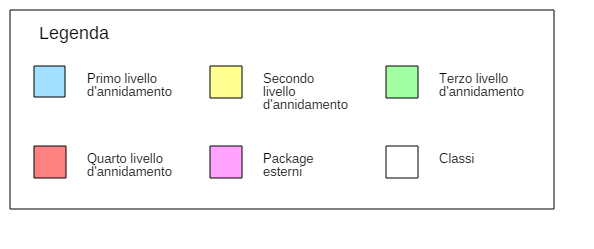
\includegraphics[scale=0.3]{Legenda.png}
			\caption{Legenda}
		\end{figure}
            \subsubsection{Server}
        	Il server di \emph{Actorbase} è composto da due package principali: il package \textbf{Core} e il package \textbf{API}. \\
            Il package \textbf{Core} è a sua volta composto dal package \textbf{Actors}, contenente le classi che definiscono gli attori del sistema, e dal package \textbf{messages}, contenente i messaggi che gli attori possono inviarsi tra loro. \\
            Il package \textbf{API} contiene le classi che forniscono una comunicazione con i client esterni.
            \begin{figure} [H]
			\centering
			\includegraphics[scale=0.35]{Server/Package/serverALL.png}
			\caption{Server, vista Package}
		\end{figure}
        \subsubsection{Client}
        	L'architettura del Client seguirà il design pattern MVC:
            \begin{itemize}
				\item \textbf{Model:}
                	Il Model è la componente che si occupa di comunicare con il server usando i metodi del driver e di notificare la View quando avviene un cambiamento nel suo stato.
                \item \textbf{View:}
                	La View è la componente che interagisce con l'utente mediante interfaccia a linea di comando. L'utente può usare il DSL per interrogare il Model. La View esegue delle \emph{state query} sul model per avere le informazioni aggiornate.
                \item \textbf{Controller:}
                	Il Controller è la componente che esegue il parsing dei comandi del DSL inseriti nella View e li notifica al Model.			
			\end{itemize}
        
        \subsubsection{Driver}
        	Il Driver è una libreria, invocando i metodi della quale è possibile effettuare richieste TCP verso le API esposte dal Server.
            
	\newpage 
	\section{Componenti}
		\subsection{Actorbase}
			\begin{figure} [H]
			\centering
			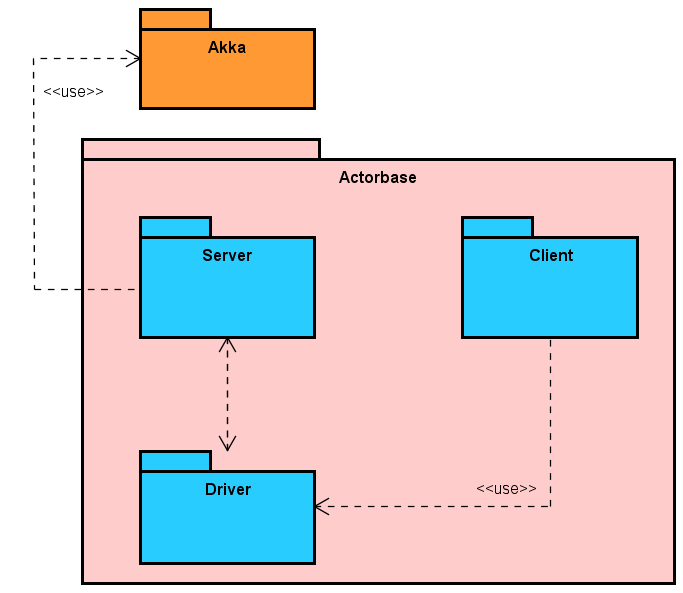
\includegraphics[scale=0.50]{Server/Package/actorbase.png}
			\caption{Componente Actorbase}
		\end{figure}
			\subsubsection{Descrizione}
				\'E il package principale del sistema. L'interazione tra i package \textbf{Server} e \textbf{Driver} definiscono una comunicazione su rete di tipo client-server. \\ Le classi definite nel package \textbf{Server} utilizzano ed estendono le classi della libreria Akka.
			\subsubsection{Package Figli}
				\begin{itemize}
					\item Actorbase.Server
					\item Actorbase.Client
					\item Actorbase.Driver
					\item Actorbase.Akka
				\end{itemize}
		\subsection{Actorbase.Server}
			\begin{figure} [H]
			\centering
			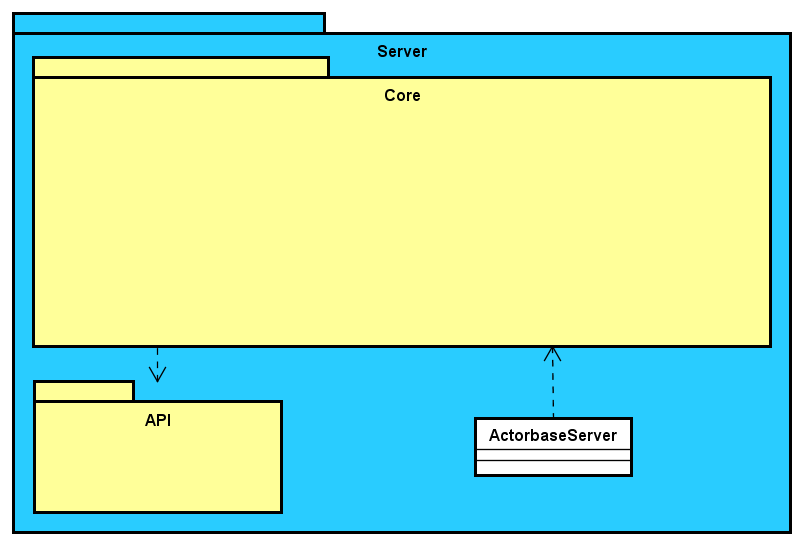
\includegraphics[scale=0.50]{Server/Package/ServerLevel.png}
			\caption{Componente Actorbase.Server}
			\end{figure}
			\subsubsection{Descrizione}
				Package per la componente lato server del sistema. \'E composto dai packages \textbf{Core} ed \textbf{API} e dalla classe \emph{ActorbaseServer}.
			\subsubsection{Package Figli}
				\begin{itemize}
					\item Actorbase.Server.Core
					\item Actorbase.Server.API
				\end{itemize}
			\subsubsection{Classi}
			\begin{itemize}
				\item Actorbase.Server.ActorbaseServer
			\end{itemize}
		\subsection{Actorbase.Server.API}
			\begin{figure} [H]
			\centering
			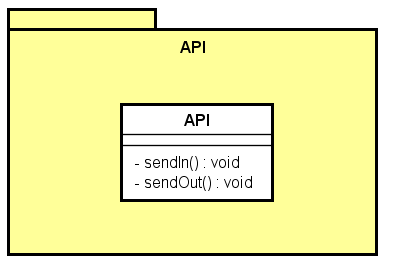
\includegraphics[scale=0.70]{Server/Package/APILevel.png}
			\caption{Componente Actorbase.Server.API}
			\end{figure}
			\subsubsection{Descrizione}
				Package contenenti le classi che definiscono le API attraverso cui i client possono interfacciarsi all'istanza di un server del sistema.
			\subsubsection{Classi}
			\begin{itemize}
				\item Actorbase.Server.API.API
			\end{itemize}
			
		\subsection{Actorbase.Server.Core}
			\begin{figure} [H]
			\centering
			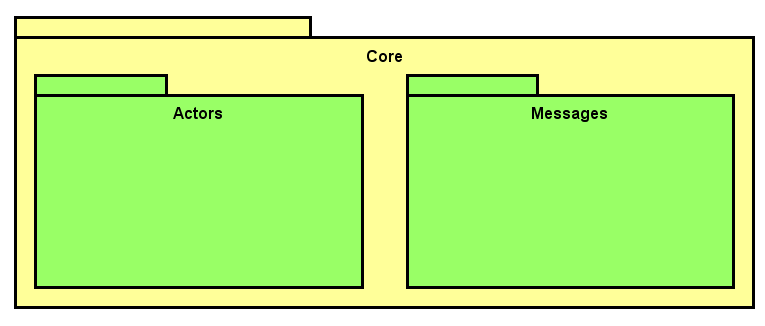
\includegraphics[scale=0.55]{Server/Package/CoreLevel.png}
			\caption{Componente Actorbase.Server.Core}
			\end{figure}
			\subsubsection{Descrizione}
				Il package contiene le componenti che costituiscono il nucleo del sistema logico lato server. \'E composto da due package: \textbf{Actors} e \textbf{Messages}
			\subsubsection{Package figli}
			\begin{itemize}
				\item Actorbase.Server.Core.Actors
				\item Actorbase.Server.Core.Messages
			\end{itemize}
			
		\subsection{Actorbase.Server.Core.Actors}
			\begin{figure} [H]
			\centering
			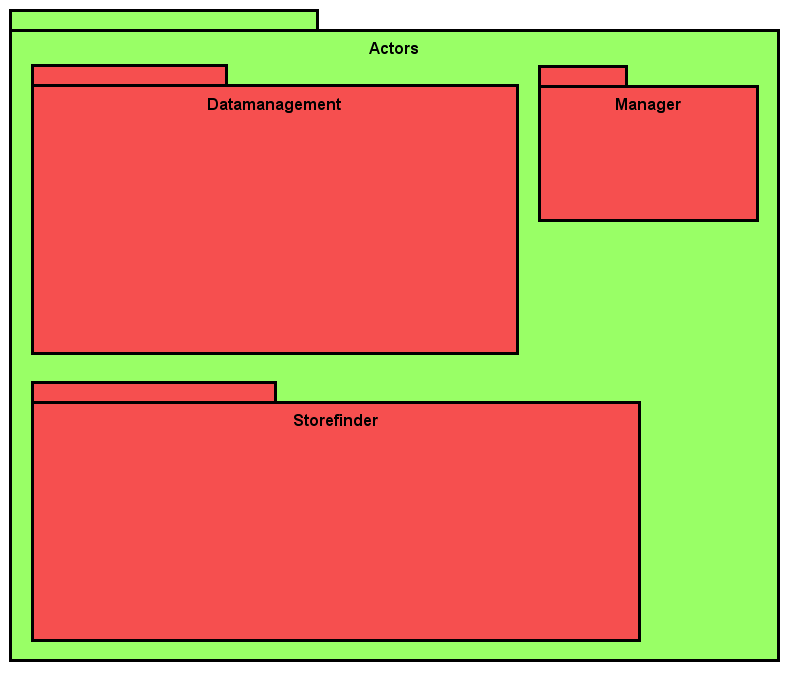
\includegraphics[scale=0.50]{Server/Package/ActorsLevel.png}
			\caption{Componente Actorbase.Server.Core.Actors}
			\end{figure}
			\subsubsection{Descrizione}
				Il package contiene le componenti che costituiscono i diversi attori definiti nel sistema. I package che lo compongono definiscono le diverse categorie degli attori.
			\subsubsection{Package figli}
			\begin{itemize}
				\item Actorbase.Server.Core.Actors.DataManagement
				\item Actorbase.Server.Core.Actors.Manager
				\item Actorbase.Server.Core.Actors.StoreFinder
			\end{itemize}
			
			\subsection{Actorbase.Server.Core.Actors.DataManagement}
			\begin{figure} [H]
			\centering
			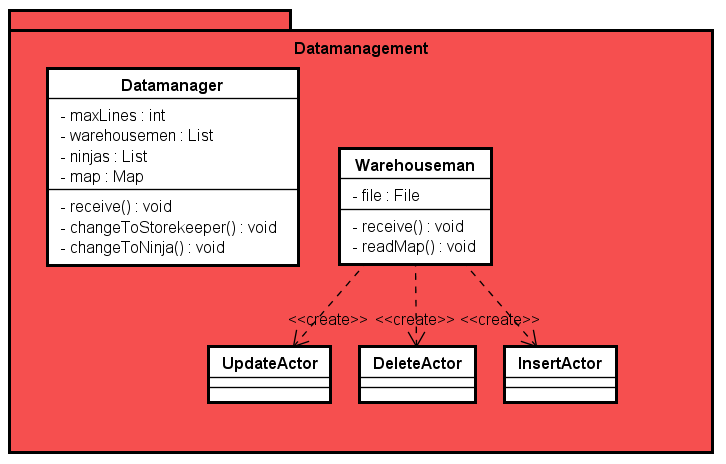
\includegraphics[scale=0.55]{Server/Package/DatamanagementLevel.png}
			\caption{Componente Actorbase.Server.Core.Actors.DataManagement}
			\end{figure}
			\subsubsection{Descrizione}
				All'interno di questo package sono definite le classi che rappresentano gli attori che si occupano direttamente della gestione dei dati.
			\subsubsection{Classi}
			\begin{itemize}
				\item Actorbase.Server.Core.Actors.DataManagement.DataManager
				\item Actorbase.Server.Core.Actors.DataManagement.WareHouseMan
				\item Actorbase.Server.Core.Actors.DataManagement.UpdateActor
				\item Actorbase.Server.Core.Actors.DataManagement.DeleteActor
				\item Actorbase.Server.Core.Actors.DataManagement.InsertActor
			\end{itemize}
			
		\subsection{Actorbase.Server.Core.Actors.Manager}
			\begin{figure} [H]
			\centering
			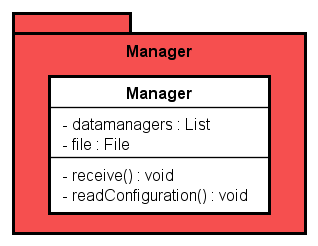
\includegraphics[scale=0.65]{Server/Package/ManagerLevel.png}
			\caption{Componente Actorbase.Server.Core.Actors.Manager}
			\end{figure}
			\subsubsection{Descrizione}
				All'interno di questo package sono definite le classi che rappresentano gli attori che si occupano della gestione di altri attori e dei vincoli presenti su di essi.
			\subsubsection{Classi}
			\begin{itemize}
				\item Actorbase.Server.Core.Actors.Manager.Manager
			\end{itemize}
			
		\subsection{Actorbase.Server.Core.Actors.StoreFinder}
			\begin{figure} [H]
			\centering
			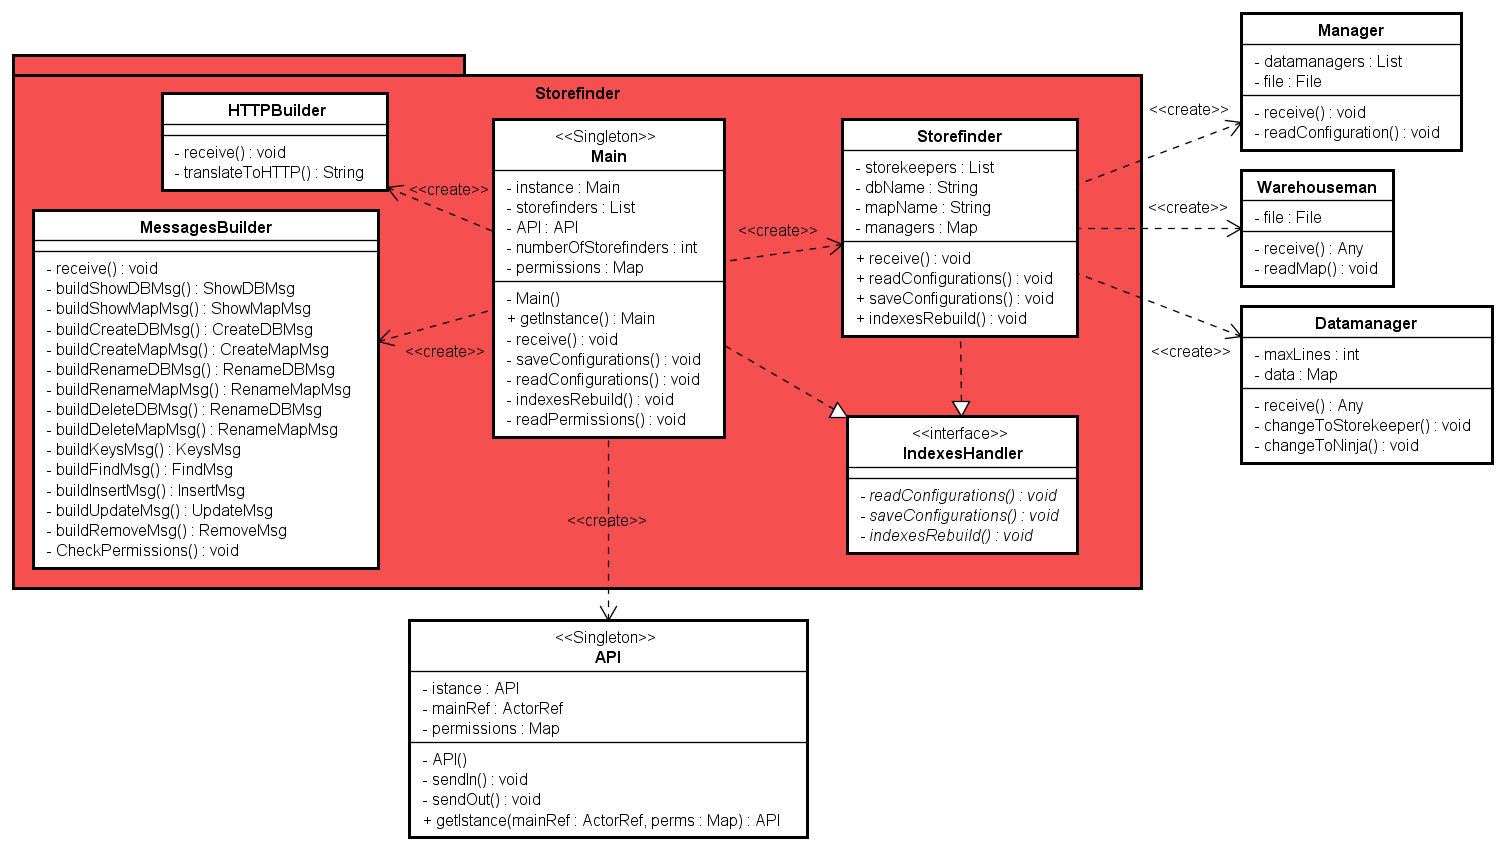
\includegraphics[width=\textwidth]{Server/Package/StorefinderLevel.png}
			\caption{Componente Actorbase.Server.Core.Actors.StoreFinder}
			\end{figure}
			\subsubsection{Descrizione}
				All'interno di questo package sono definite le classi che rappresentano gli attori che si occupano dell'indicizzazione degli altri attori presenti e del corretto instradamento dei messaggi.
			\subsubsection{Classi}
			\begin{itemize}
				\item Actorbase.Server.Core.Actors.StoreFinder.StoreFinder
				\item Actorbase.Server.Core.Actors.StoreFinder.Main
				\item Actorbase.Server.Core.Actors.StoreFinder.HTTPBuilder
				\item Actorbase.Server.Core.Actors.StoreFinder.MessageBuilder
			\end{itemize}
			\subsubsection{Interfacce}
			\begin{itemize}
				\item Actorbase.Server.Core.Actors.StoreFinder.IndexesHandler
			\end{itemize}
		
		\subsection{Actorbase.Server.Core.Messages}
			\begin{figure} [H]
			\centering
			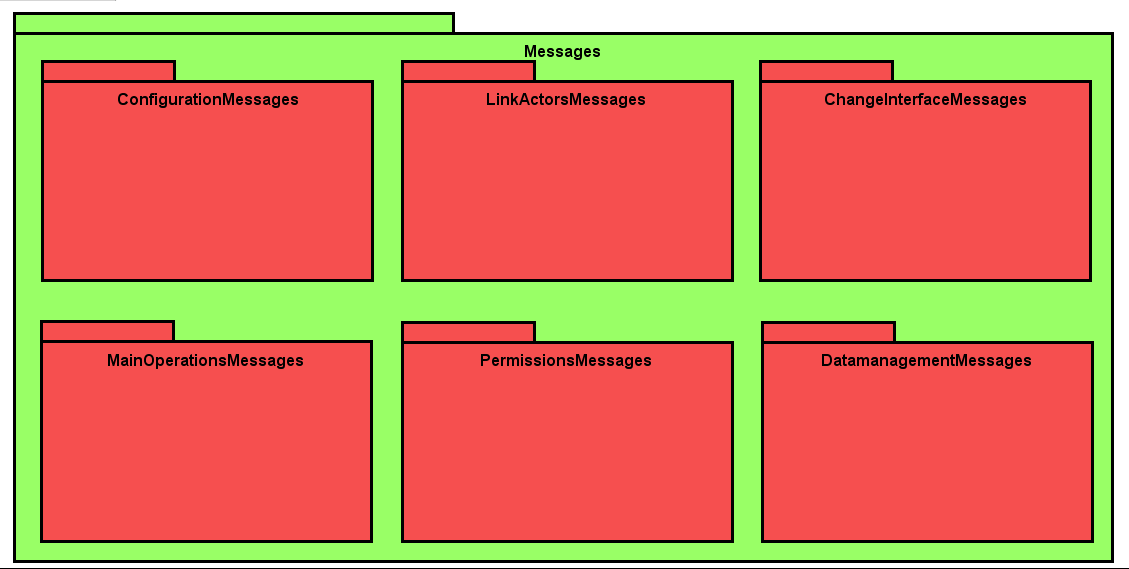
\includegraphics[scale=0.55]{Server/Package/MessagesLevel.png}
			\caption{Componente Actorbase.Server.Core.Messages}
			\end{figure}
			\subsubsection{Descrizione}
				All'interno di questo package sono definite le componenti che rappresentano i messaggi che i diversi attori del sistema possono inviarsi tra loro.
			\subsubsection{Package Figli}
			\begin{itemize}
				\item Actorbase.Server.Core.Messages.ConfigurationMessages
				\item Actorbase.Server.Core.Messages.PermissionMessages
				\item Actorbase.Server.Core.Messages.LinkActorsMessages
				\item Actorbase.Server.Core.Messages.MainOperationMessages
				\item Actorbase.Server.Core.Messages.DataManagementMessages
				\item Actorbase.Server.Core.Messages.ChangeInterfaceMessages
			\end{itemize}
			
			\subsection{Actorbase.Server.Core.Messages.ConfigurationMessages}
			\begin{figure} [H]
			\centering
			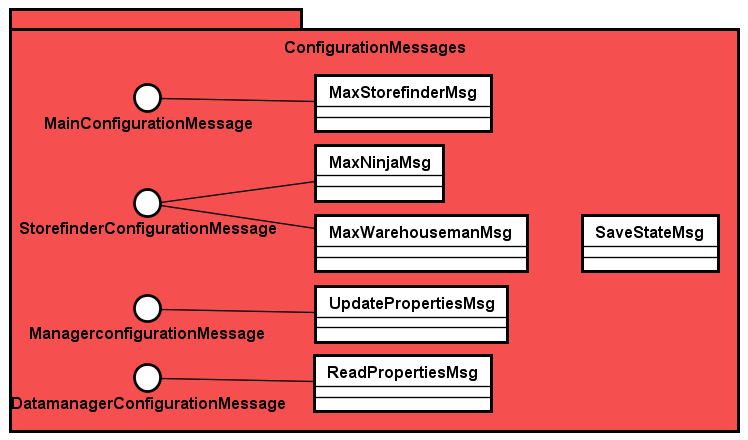
\includegraphics[scale=0.55]{Server/Package/ConfigurationMessagesLevel.png}
			\caption{Componente Actorbase.Server.Core.Messages.ConfigurationMessages}
			\end{figure}
			\subsubsection{Descrizione}
				All'interno di questo package sono definite le classi e le interfacce che rappresentano i messaggi relativi ad operazioni di configurazione delle impostazioni del server.
			\subsubsection{Classi}
			\begin{itemize}
				\item Actorbase.Server.Core.Messages.ConfigurationMessages.MaxStoreFinderMsg
				\item Actorbase.Server.Core.Messages.ConfigurationMessages.MaxNinjaMsg
				\item Actorbase.Server.Core.Messages.ConfigurationMessages.MaxWarehousemanMsg
				\item Actorbase.Server.Core.Messages.ConfigurationMessages.UpdatePropertiesMsg
				\item Actorbase.Server.Core.Messages.ConfigurationMessages.ReadPropertiesMsg
				\item Actorbase.Server.Core.Messages.ConfigurationMessages.SaveStateMsg
			\end{itemize}
			\subsubsection{Interfacce}
			\begin{itemize}
				\item Actorbase.Server.Core.Messages.ConfigurationMessages.MainConfigurationMessage
				\item Actorbase.Server.Core.Messages.ConfigurationMessages.StoreFinderConfigurationMessage
				\item Actorbase.Server.Core.Messages.ConfigurationMessages.ManagerConfigurationMessage
				\item Actorbase.Server.Core.Messages.ConfigurationMessages.DataManagerConfigurationMessage
			\end{itemize}
			
			\subsection{Actorbase.Server.Core.Messages.PermissionMessages}
			\begin{figure} [H]
			\centering
			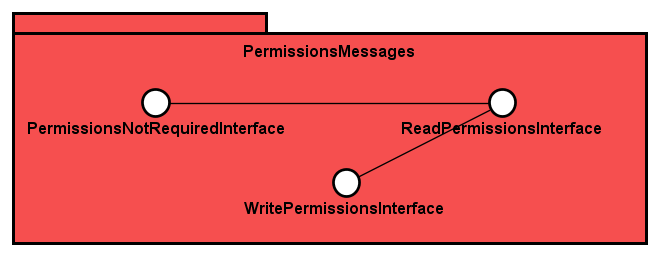
\includegraphics[scale=0.65]{Server/Package/PermissionsMessagesLevel.png}
			\caption{Componente Actorbase.Server.Core.Messages.PermissionMessages}
			\end{figure}
			\subsubsection{Descrizione}
				All'interno di questo package sono definite le interfacce che rappresentano i diversi gradi di permesso che un'operazione richiede. Un'operazione può infatti richiedere i permessi di lettura, scrittura o nessun permesso. Ogni messaggio relativo ad un'operazione richiedibile da un client estende una di queste interfacce.
			\subsubsection{Interfacce}
			\begin{itemize}
				\item Actorbase.Server.Core.Messages.PermissionMessages.PermissionsNotRequiredInterface
				\item Actorbase.Server.Core.Messages.PermissionMessages.ReadPermissionsInterface
				\item Actorbase.Server.Core.Messages.PermissionMessages.WritePermissionsInterface
			\end{itemize}
			
			\subsection{Actorbase.Server.Core.Messages.LinkActorsMessages}
			\begin{figure} [H]
			\centering
			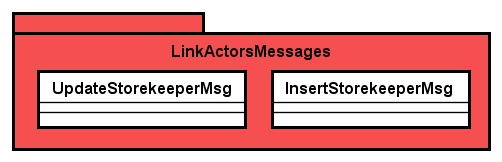
\includegraphics[scale=0.65]{Server/Package/LinkActorsMessagesLevel.png}
			\caption{Componente Actorbase.Server.Core.Messages.LinkActorsMessages}
			\end{figure}
			\subsubsection{Descrizione}
				All'interno di questo package sono definite le classi che rappresentano i messaggi relativi alla gestione dei collegamenti tra diversi attori.
			\subsubsection{Classi}
			\begin{itemize}
				\item Actorbase.Server.Core.Messages.LinkActorsMessages.UpdateStoreKeeperMsg
				\item Actorbase.Server.Core.Messages.LinkActorsMessages.InsertStoreKeeperMsg
			\end{itemize}
			
			\subsection{Actorbase.Server.Core.Messages.MainOperationMessages}
			\begin{figure} [H]
			\centering
			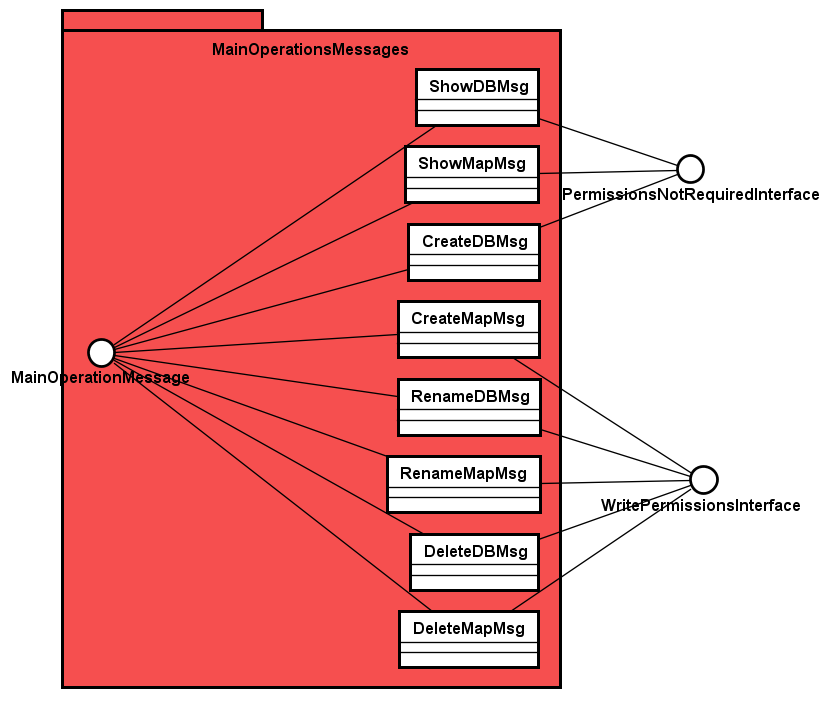
\includegraphics[scale=0.55]{Server/Package/MainOperationsMessagesLevel.png}
			\caption{Componente Actorbase.Server.Core.Messages.MainOperationMessages}
			\end{figure}
			\subsubsection{Descrizione}
				All'interno di questo package sono definite le classi e le interfacce che rappresentano i messaggi relativi ad operazioni che non richiedono l'invio di ulteriori messaggi ad attori che gestiscono i dati direttamente.
			\subsubsection{Classi}
			\begin{itemize}
				\item Actorbase.Server.Core.Messages.MainOperationMessages.ShowDBMsg
				\item Actorbase.Server.Core.Messages.MainOperationMessages.ShowMapMsg
				\item Actorbase.Server.Core.Messages.MainOperationMessages.CreateDBMsg
				\item Actorbase.Server.Core.Messages.MainOperationMessages.CreateMapMsg
				\item Actorbase.Server.Core.Messages.MainOperationMessages.RenameDBMsg
				\item Actorbase.Server.Core.Messages.MainOperationMessages.RenameMapMsg
				\item Actorbase.Server.Core.Messages.MainOperationMessages.DeleteDBMsg
				\item Actorbase.Server.Core.Messages.MainOperationMessages.DeleteMapMsg
			\end{itemize}
			\subsubsection{Interfacce}
			\begin{itemize}
				\item Actorbase.Server.Core.Messages.MainOperationMessages.MainOperationMessage
			\end{itemize}
			
		\subsection{Actorbase.Server.Core.Messages.DataManagerOperationMessages}
			\begin{figure} [H]
			\centering
			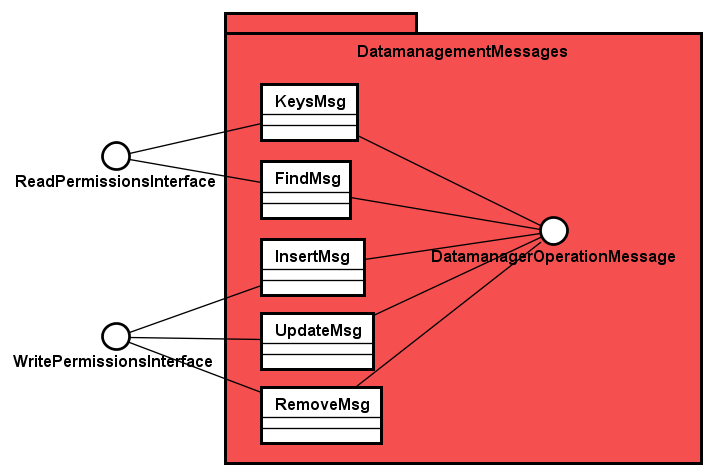
\includegraphics[scale=0.50]{Server/Package/DatamanagementMessagesLevel.png}
			\caption{Componente Actorbase.Server.Core.Messages.DataManagerOperationMessages}
			\end{figure}
			\subsubsection{Descrizione}
				All'interno di questo package sono definite le classi e le interfacce che rappresentano i messaggi relativi ad operazioni che richiedono l'invio di tali messaggi anche ad attori che gestiscono i dati direttamente.
			\subsubsection{Classi}
			\begin{itemize}
				\item Actorbase.Server.Core.Messages.DataManagerOperationMessages.KeysMsg
				\item Actorbase.Server.Core.Messages.DataManagerOperationMessages.FindMsg
				\item Actorbase.Server.Core.Messages.DataManagerOperationMessages.InsertMsg
				\item Actorbase.Server.Core.Messages.DataManagerOperationMessages.UpdateMsg
				\item Actorbase.Server.Core.Messages.DataManagerOperationMessages.RemoveMsg
			\end{itemize}
			\subsubsection{Interfacce}
			\begin{itemize}
				\item Actorbase.Server.Core.Messages.DataManagerOperationMessages.DataManagerOperationMessage
			\end{itemize}
			
			\subsection{Actorbase.Server.Core.Messages.ChangeInterfaceMessages}
			\begin{figure} [H]
			\centering
			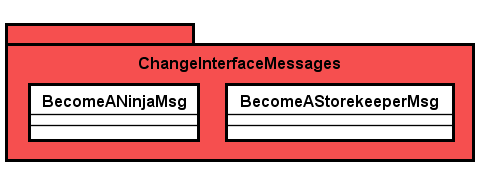
\includegraphics[scale=0.65]{Server/Package/ChangeInterfaceMessagesLevel.png}
			\caption{Componente Actorbase.Server.Core.Messages.ChangeInterfaceMessages}
			\end{figure}
			\subsubsection{Descrizione}
				All'interno di questo package sono definite le classi e le interfacce che rappresentano i messaggi inviabili per effettuare operazioni di cambio interfaccia per gli attori che supportano tale funzionalità.
			\subsubsection{Classi}
			\begin{itemize}
				\item Actorbase.Server.Core.Messages.ChangeInterfaceMessages.BecomeNinjaMsg
				\item Actorbase.Server.Core.Messages.ChangeInterfaceMessages.BecomeStoreKeeperMsg
			\end{itemize}
			
	\newpage
	\section{Classi}	
	
	\newpage 
	\section{Diagrammi delle attività}
	
	\newpage 
	\section{Design pattern}
	
	\newpage 
	\section{Stime di fattibilità e di bisogno di risorse}
	
	\newpage 
	\section{Tracciamento}
		\subsection{Tracciamento componenti-requisiti}
		\subsection{Tracciamento requisiti-componenti}
		
	\newpage 
	\section{Appendice}
	\subsection{Descrizione Desing Pattern}
	Segue, per ogni Desing Pattern utilizzato, la descrizione dello scopo, motivazione e applicabilità.
	\subsubsection{Event-driven}
				\begin{figure}[H]
					\centering
					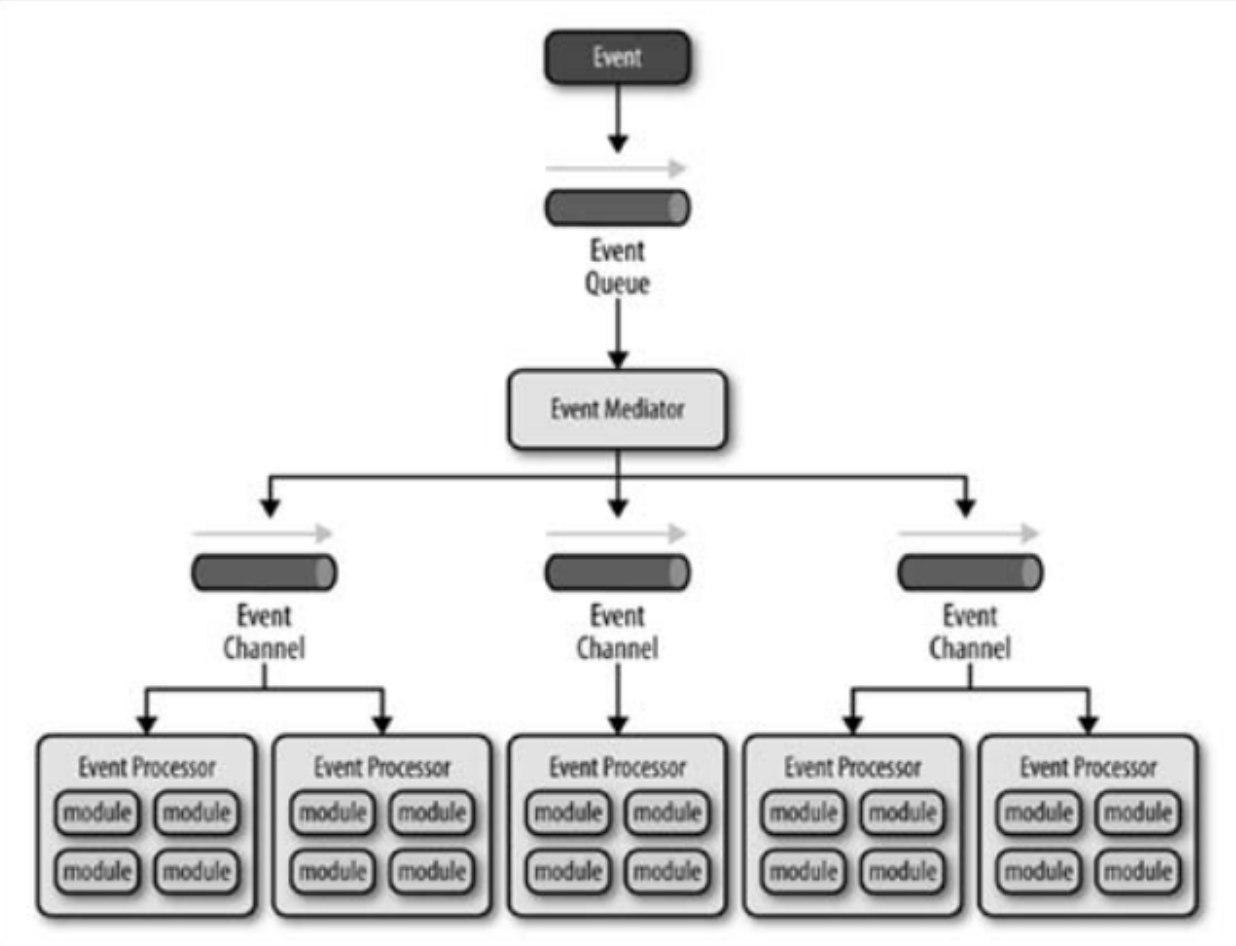
\includegraphics[scale=0.65]{schemaevent-driven.jpg}
					\caption{Diagramma del Desing Pattern Event-driven}
				\end{figure}
            \begin{itemize}
				\item \textbf{Scopo:}
					Produrre applicazioni molto scalabili e processare eventi asincroni disaccoppiati.
                \item \textbf{Motivazione:} Gestire le richieste che vengono volte all' applicativo tramite eventi processati in modo asincrono.
                \item \textbf{Applicabilità:}
                	Gestione di eventi attraverso l'utilizzo di un mediatore e elaboratori di eventi		
			\end{itemize}
	\subsubsection{MVC}
				\begin{figure}[H]
					\centering
					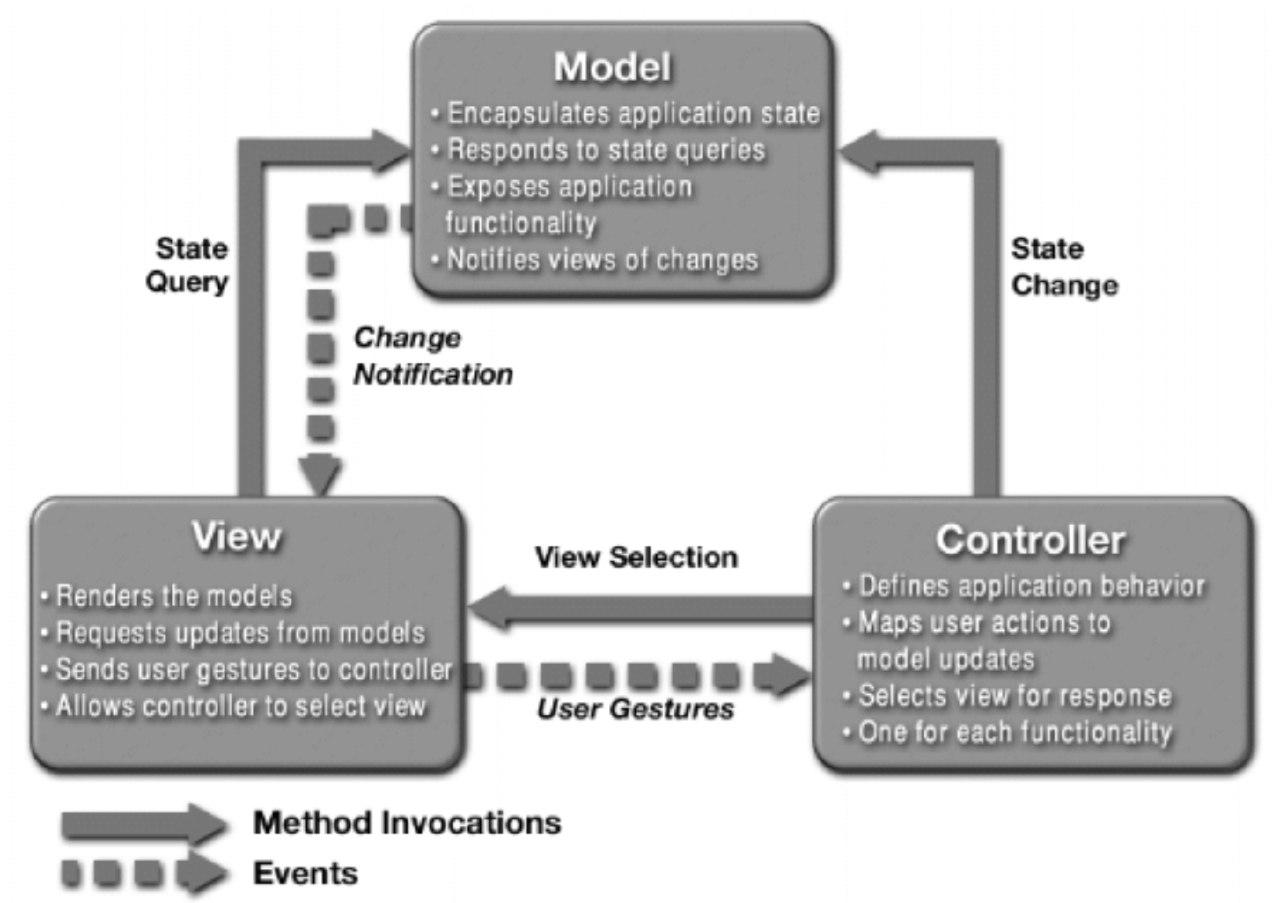
\includegraphics[scale=0.65]{schemaMVC.jpg}
					\caption{Diagramma del Desing Pattern MVC}
				\end{figure}
            \begin{itemize}
				\item \textbf{Scopo:}
					Disaccoppiamento delle seguenti componenti:
					\begin{itemize}
						\item Model regole di accesso e dati di business
						\item View rappresentazione grafica
						\item Controller reazioni della UI agli input utente
					\end{itemize}
                \item \textbf{Motivazione:}
                	Lo scopo di molti applicativi è di recuperare dati e mostrarli all'Utente. Si è visto che la migliore soluzione di questo scopo è dividere la modellazione del dominio, la presentazione e le reazioni basate sugli input degli utenti i tre classi separate, esistono vari desing pattern che svolgono questa separazione, uno di questi è MVC; 
                \item \textbf{Applicabilità:}
					\begin{itemize}
						\item Applicazioni che devono presentare attraverso una UI un insieme di informazioni
						\item Le persone responsabili dello sviluppo hanno compentenze differenti
					\end{itemize}
                	 		
			\end{itemize}
	\subsubsection{Command}
				\begin{figure}[H]
					\centering
					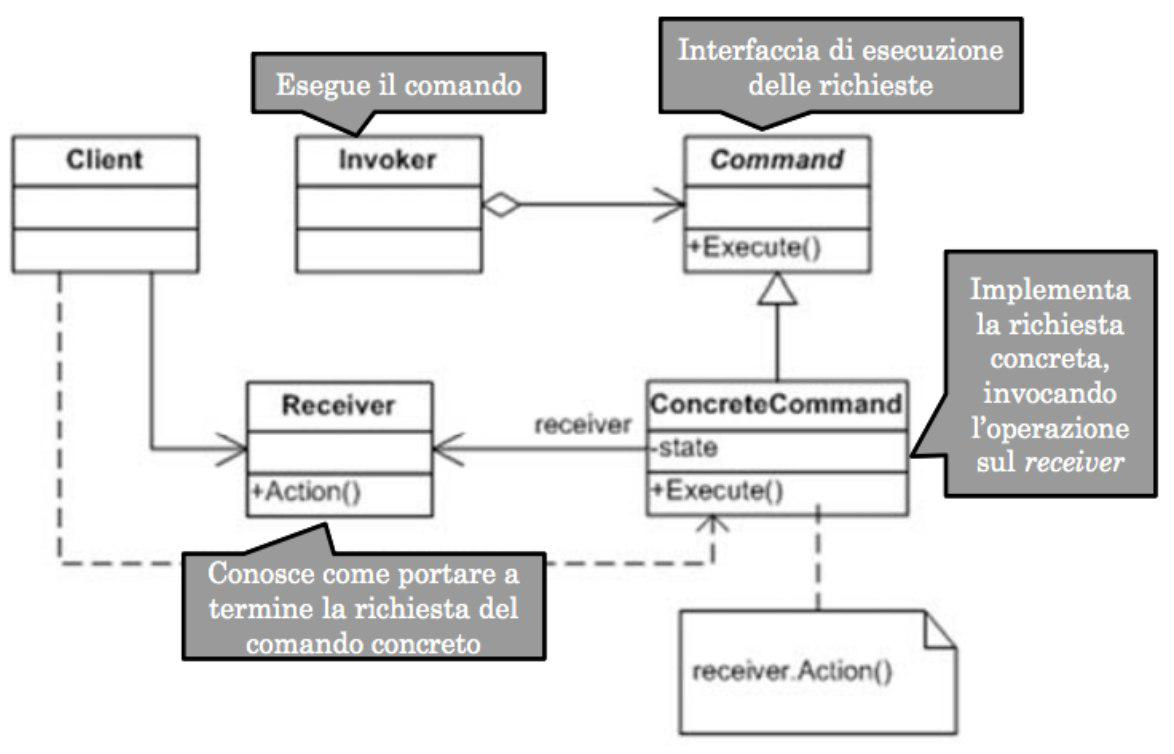
\includegraphics[scale=0.65]{schemacomand.jpg}
					\caption{Diagramma del Desing Pattern Command}
				\end{figure}
            \begin{itemize}
				\item \textbf{Scopo:}Incapsulare una richiesta in un oggetto, cosicché i client siano indipendenti dalle richieste 
                \item \textbf{Motivazione:}
                Risolvere la necessità di gestire richieste di sui non si conoscono i particolari, tramite una classe astratta, Command, che definisce un interfaccia per eseguire la richiesta
                \item \textbf{Applicabilità:}
					\begin{itemize}
						\item Parametrizzazione di oggetti sull'azione da eseguire
						\item Specificare, accordare ed eseguire richieste molteplici volte
						\item Supporto ad operazioni di Undo e Redo
						\item Supporto a transazione, un comando equivale ad una operazione atomica
					\end{itemize}		
			\end{itemize}
				
	
	\cleardoublepage
	\addcontentsline{toc}{section}{\listfigurename}
	\listoffigures
	
	\cleardoublepage
	\addcontentsline{toc}{section}{\listtablename}
	\listoftables
		
\end{document}